Sebuah SDLC yang terlahir dari kekuasaan tirranis waterfall. \emph{Rapid Application Development} atau RAD,
bertujuan untuk memberi alternatif pada waterfall yang lebih flexible, user oriented, dan pengembangan iterative,
dimana model RAD memungkinkan pengembangan \emph{software} yang lebih cepat dibanding model waterfall.

\subsection{Rencana Baru}
Rapid Application Development adalah metodologi pengembangan perangkat lunak 
yang diperkenalkan pada tahun 1990-an dan disajikan dalam bentuk buku \emph{Rapid Application Development}
oleh ahli teknologi informasi James Martin. Sebuah reaksi terhadap metodologi yang sudah 
mapan saat itu yang menekankan pada pengumpulan persyaratan yang cermat dan 
berkepanjangan sebelum pengembangan perangkat lunak yang sebenarnya dimulai.\cite{bestpricecomputer}

Walau James Martin bukan "pencipta" dari SDLC RAD, ada beberapa contoh penggunaan prinsip-prinsip
RAD seperti Barry Boehman dengan pembuatan model Spiral. James Martin lah yang menformalisasikan
RAD sebagai model SDLC tersendiri.

\subsection{Apa Itu RAD?}
Rapid Application Development (RAD) atau \emph{Rapid Prototyping} adalah model 
proses pembangunan perangkat lunak yang tergolong dalam teknik incremental (bertingkat). 
RAD menekankan pada siklus pembangunan pendek, singkat, dan cepat. Waktu yang singkat 
adalah batasan yang penting untuk model ini. Rapid application development menggunakan 
metode iteratif (berulang) dalam mengembangkan sistem dimana \emph{working model} 
sistem dikonstruksikan di awal tahap pengembangan dengan tujuan menetapkan kebutuhan (requirement) 
user dan selanjutnya disingkirkan. Working model digunakan kadang-kadang saja sebagai basis desain dan implementasi sistem final.\cite{anakkos}

\subsection{Sruktur}
Fondasi RAD sebagai system yang sangat flexible, terlihat sangat jelas disaat kita melihat
\emph{Life Cycle} model tersebut\cite{codebots} :

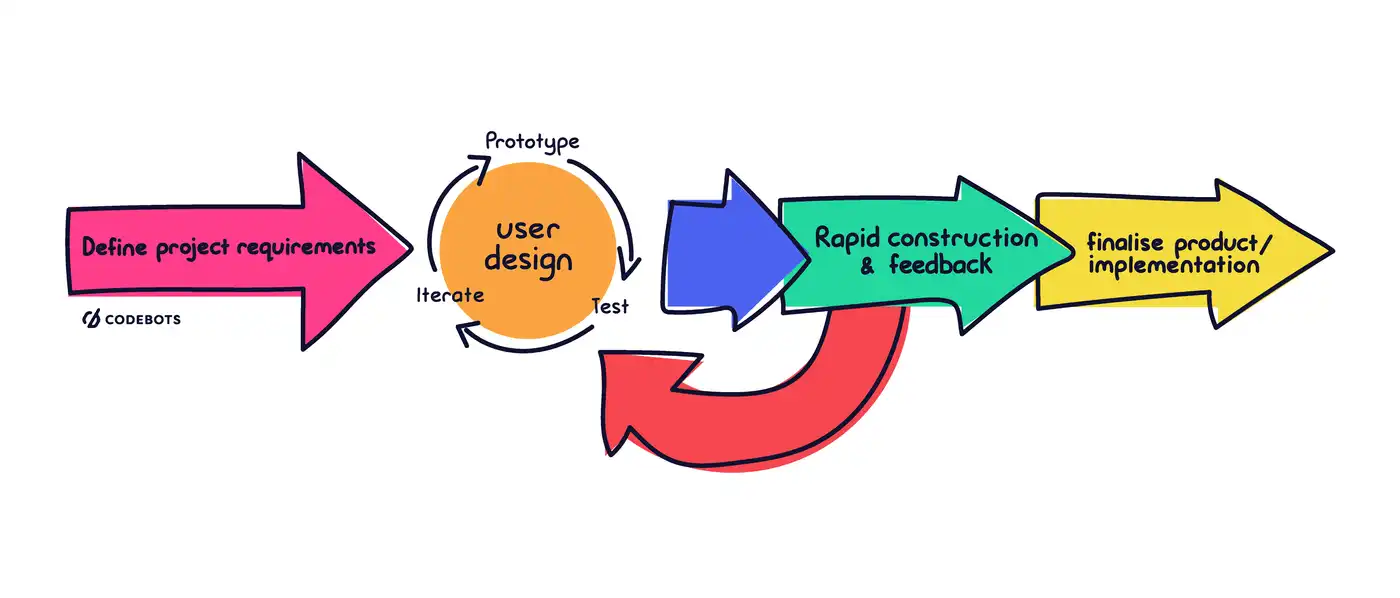
\includegraphics[width=1.05\textwidth, angle=-90]{images/rad-cycle.png}\newline

\begin{enumerate}
    \item \emph{Define project requirements}:\\
    \textbf{Fase awal dimana semua pihak terkait mendefinisikan requirements yang dibutuhkan secara besar.}

    \item \emph{Prototype}:\\
    \textbf{proses interaktif kontinu yang memungkinkan pengguna untuk memahami, memodifikasi, dan pada akhirnya menyetujui model kerja sistem yang memenuhi kebutuhan mereka.}

    \item \emph{Rapid Construction and Feedback Gathering}:\\
    \textbf{Rapid Construction adalah tempat pengkodean aplikasi, pengujian sistem, dan integrasi unit, mengubah prototipe dan sistem beta menjadi model kerja.}

    \item \emph{Finalise product / implementation}:\\
    \textbf{Fase terakhir dari Rapid Application Development, di mana developer mengatasi utang teknis yang timbul dalam pembuatan prototipe awal, mengoptimalkan implementasi untuk meningkatkan stabilitas dan maintenance saat mereka menyelesaikan produk untuk diluncurkan.}
\end{enumerate}

\subsection{RAD vs Tradisi}
Table berikut akan menjelaskan perbedaan sistem RAD dengan sistem SDLC tradisional\cite{wavemaker} :

\newpage

\begin{center}
    \begin{tabular}{||c c c ||} 
     \hline
     Parameter & RAD & Tradisional SDLC \\ [0.5ex] 
     \hline\hline
     Proses Pengembangan Applikasi & Inkremental dan Iteratif & Linear dan Prediktif\\ 
     \hline
     Struktur Team & Tim yang kecil dan flexible & Tim yang besar dan kaku \\
     \hline
     Produktivitas dan Flexibilitas & Tinggi : struktur iteratif & Rendah : struktur linear\\
     \hline
     Dokumentasi & Minimalist & Full Spesifikasi \\
     \hline
     Waktu dan Estimasi Harga & Variable & Fixed \\
     \hline
     Uji Coba & Extensive & Minimal \\
     \hline
     Interaksi Pengguna Akhir & Setiap fase development & Hanya awal\\
     \hline
    \end{tabular}
\end{center}    

\newpage

Dari tabel tersebut, kita bisa menyimpulkan bahwa perbedaan paling dominan dari kedua sistem tersebut
antara flexibitas dengan keteguhan, iterasi dengan lineariti, dan komunikasi konstant dengan
komunikasi kecil.

\subsection{Kelebihan/Kekurangan RAD}
Berikut adalah beberapa kelebihan sistem RAD:\cite[See p.75]{agustinus}

\begin{enumerate}
    \item Proses pengiriman menjadi lebih mudah, hal ini dikarenakan proses pembuatan lebih banyak menggunakan potongan - potongan script.
    \item Mudah untuk diamati karena menggunakan model prototype, sehingga user lebih mengerti akan sistem yang dikembangkan.
    \item Lebih fleksibel karena pengembang dapat melakukan proses desain ulang pada saat yang bersamaan.
    \item Mampu meminimalkan kesalahan-kesalahan dengan menggunakan alat-alat bantuan (CASE tools).
    \item Mempercepat waktu pengembangan sistem secara keseluruhan karena cenderung mengabaikan kualitas.
\end{enumerate}

Berikut adalah beberapa kekurangan sistem RAD:

\begin{enumerate}
    \item Membutuhkan komitmen tingkat tinggi dari semua pihak.
    \item Memerlukan sistem modular dan sulit untuk proyek berskala besar.
    \item Ketelitian menjadi berkurang karena tidak menggunakan metode yang formal dalam melakukan pengkodean.
    \item Kesulitan melakukan pengukuran mengenai kemajuan proses.
    \item Menuntut fokus antarmuka karena fokusnya pada protoyping.
\end{enumerate}

\subsection{Untuk Siapa sih?}
RAD adalah metode yang baik untuk lingkungan yang bergerak 
cepat dengan tim berpengalaman yang memiliki anggaran untuk 
alat pengembangan aplikasi yang cepat, seperti \emph{Low Code Platform} 
dan generator kode. RAD sangat berguna untuk usaha kecil 
yang menghasilkan produk inovatif di pasar yang kompetitif 
dan membutuhkan keterlibatan bisnis yang tinggi. Pendekatan \emph{on-the-fly} 
mengakomodasi perubahan kebutuhan yang tidak terduga. Ketika proyek 
memiliki tenggat waktu yang ketat, metode pengembangan aplikasi yang cepat 
membuat tim bertanggung jawab untuk memberikan produk yang berfungsi secepat mungkin.

Pertimbangkan daftar berikut ini untuk menilai apakah sistem RAD tepat untuk Anda.\cite{codebots}

\begin{enumerate}
    \item Apakah Anda memiliki tim yang berpengalaman yang dapat berkomitmen pada proses pengembangan yang intensif dan berkelanjutan yang melibatkan komunikasi tingkat tinggi?
    \item Apakah klien Anda terbuka terhadap sistem ini, dan tingkat keterlibatan langsung yang diperlukan? Jika tidak, gangguan komunikasi dapat menyebabkan proyek gagal.
    \item Apakah klien Anda bersedia mematuhi jadwal proyek dan jadwal penyelesaian model? Semua pihak berkepentingan harus terlibat untuk menerapkan metodologi ini secara efektif.
    \item Dapatkah sistem dimodularisasi dalam jangka waktu 2-3 bulan?
    \item Apakah Anda memiliki alat komunikasi dan pengembangan serta perangkat lunak yang tepat untuk menerapkan RAD secara efektif? Jika tidak, apakah Anda memiliki anggaran untuk membeli alat yang dibutuhkan, termasuk anggota tim ahli tambahan jika diperlukan?
\end{enumerate}